\documentclass[crop,tikz]{standalone}

\usepackage{amsmath}
\usepackage{pgfplots}
\usepackage[locale=DE]{siunitx}
\tikzset{>=latex}

\pgfplotsset{
  inverted/.style = {
    every axis legend/.append style={
      draw=white,
      fill=hardblack,
      text=white
    }
  },
  every non boxed x axis/.append style={
    axis line style={-latex}
  },
  every non boxed y axis/.append style={
    axis line style={-latex}
  }
}

\begin{document}
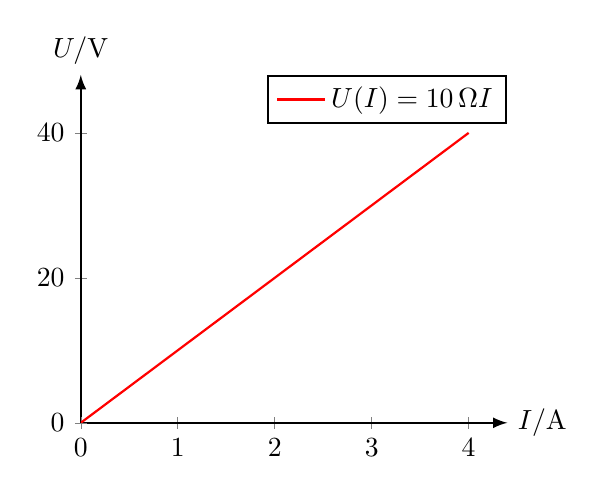
\begin{tikzpicture}
\pgfmathsetmacro{\resistance}{10}
\begin{axis}[
  thick,
  width=7cm,
  height=6cm,
  domain={0}:{4},
  samples=100,
  smooth,
  axis y line=middle,
  axis x line=middle,
  xlabel={$I/\si{\A}$},
  ylabel={$U/\si{\V}$},
  xlabel style={right},
  ylabel style={above},
  xmin=0, xmax=4.4,
  ymin=0, ymax=48,
  extra x ticks={0},
  extra y ticks={0},
  legend cell align={left},
  legend style={at={(1,1)},anchor=north east}
  ]
  \addplot[red] { \resistance*x };
  \addlegendentry{$U(I)=\SI{\resistance}{\ohm}I$};
\end{axis}
\end{tikzpicture}
\end{document}
